\chapter{Tables, pictures, programs, formulas}

The use of tables and graphs/figures in technical text has some common rules and 
some specific ones. We do not present tables and graphs/figures directly in the 
text, but we place them either on separate pages or in a reserved place at the 
top or bottom of regular pages. \LaTeX\ will take care of the placement of 
floating graphs and tables automatically.

Graphs/figures and tables are numbered and equipped with a legend. The legend 
should describe the content of the graph or table in such detail that the reader 
understands them without a thorough study of the text of the work.

There must be a numerical reference to the table and graph/figure in the text (a 
dynamic cross-reference mechanism, which is part of \LaTeX, can be strongly 
recommended). At the appropriate place in the text, we then summarize the most 
important conclusions that can be drawn from a table or graph. The text should 
be legible and understandable even without looking at the tables and graphs, and 
the tables and graphs should be understandable even without reading the text in 
detail.

We refer to tables and graphs, if possible, indirectly during the normal flow of 
text; instead \emph{\uv{Table~\ref{tab03:Nejaka} shows that men are on average 
about~$9,9\,\rm kg$ heavier than women}} we'd rather write \emph{\uv{Men are 
~$9,9\,\rm kg$ heavier then women (see tab.~\ref{tab03:Nejaka})}}.

\section{Tables}

\begin{table}[htbp!]

\centering
%%% The table uses the following packages:
%%%   - booktabs (\toprule, \midrule, \bottomrule)
%%%   - dcolumn (column type D: centered numbers aligned to
%%%     decimal point
%%%     Note that there are decimal points in the source code, but
%%%     commas are printed.

\caption{Maximum plausible estimates in model M.}\label{tab03:Nejaka}
\begin{tabular}{lD{.}{,}{3.2}D{.}{,}{1.2}D{.}{,}{2.3}}
\toprule
               &                & \multicolumn{1}{c}{\textbf{Standard.}}   &  \\
\textbf{Effect} & \multicolumn{1}{c}{\textbf{Estimate}} & \multicolumn{1}{c}{\textbf{deviation}$^a$} & \multicolumn{1}{c}{\textbf{P-value}} \\
\midrule
Abs. member     & -10.01 & 1.01 & \multicolumn{1}{c}{---} \\
Gender (male) & 9.89   & 5.98 & 0.098 \\
Height (cm)    & 0.78   & 0.12 & <0.001 \\
\bottomrule
\multicolumn{4}{l}{\footnotesize \textit{Pozn:}$^a$ Standard error of estimation by Monte Carlo method.}
\end{tabular}
\end{table}

The following tips specifically apply to \textbf{tables}:

\begin{itemize} %% or compactitem from package paralist

\item Never copy tables from statistical software to a thesis. Typically, 
statistical software also includes more information in tables than necessary.

\item Avoid vertical lines. Thicker horizontal lines separate the table from the 
surrounding text, including the legend, weaker horizontal lines separate the 
column headers from the table body, and the individual parts of the table from 
each other. In \LaTeX, the \texttt{booktabs} package implements this form of 
tables. If we want to significantly separate some columns from others, we insert 
a larger space between them

\item Keep the type, format and sense of the field content in a single column. 
It is not advised to enter, e.g., average and percent in the same column.

\item Avoid repeating the same field content too many times. E.g., if the column 
Variance shows the value of 0.5 in the first ten lines and 1.5 in the following 
ten lines, cancel the column. Find a different solution. E.g., one can divide 
the table to two. Alternatively, one can enter descriptive lines that inform of 
a variable value repeating in the following table section. E. g.
\emph{\uv{Variance${}=0,5$}} and below \emph{\uv{Variance${}= 1,5$}}).

\item All numbers shall have the same number of valid digits. Numbers in a table 
shall be aligned to the decimal point.

\item A~table sometimes requires the use of abbreviations that do not occur 
elsewhere. Such abbreviations may be explained in the legend or notes below the 
table. Notes below the table may also be used for an explanation of the sense of 
some columns or values.

\end{itemize}


\section{Figures}

\begin{figure}[htbp!]\centering
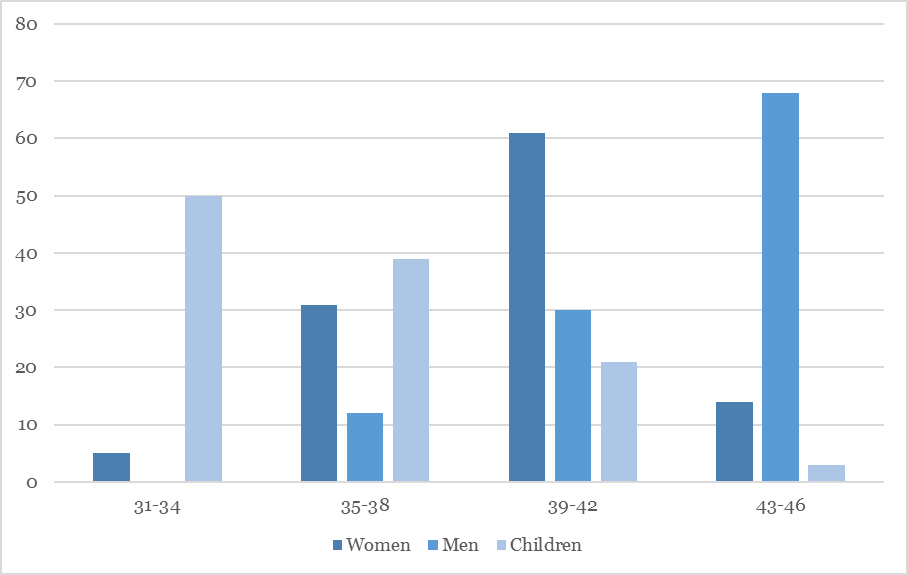
\includegraphics[width=.66\textwidth]{img/example-fig}
% Příponu není potřeba explicitně uvádět, pdflatex automaticky hledá pdf.
% Rozměry také není nutné uvádět.
\caption{Frequency of shoe size in the population of men, women and children (CZSO data, Author’s calculation)}
\label{fig:freq-shoe-size}
\end{figure}

There are several general tips for figures and diagrams.

\begin{itemize}

\item A~figure/diagram should be created in the same size as used in the thesis. 
Decreasing a large diagram leads to having unreadable labels. Increasing a small 
diagram leads to poor graphical quality.

\item The diagram axis shall be properly labelled in the thesis language. 
Missing punctuation is tolerable. If a diagram deals with, e.g., weight and 
height, the labels shall say \emph{Height [cm]} and \emph{Weight [kg]}. If the 
graph includes the function \emph{h(x)}, the axes get a label of \emph{x} and 
\emph{h(x)}. Each axis shall bear a clearly defined scale. 

\item If a two-dimensional diagram marks many points, the author should make 
sure that they do not get mixed. If the number of points is too high, the author 
should decrease the size of the symbols that refer to them or select a lower 
number of points to mark in the diagram. Diagrams with thousands of marked 
points cause problems mainly in electronic documents by increasing the file 
size. 

\item If the thesis is to be printed in black and white, the author should avoid 
using colours. Lines should be distinguished by line type (full, dotted, 
dashed…). Sections should be distinguished by distinct shades of grey or 
hatching. The sense of individual line types or hatched sections shall be 
explained either in the diagram textual legend or in a graphic legend integrated 
into the diagram. 

\item Avoid bitmap figures with a low resolution, especially JPEGs. Compression 
artifacts do not look good on paper. 

\end{itemize}


\section{Source codes}

Algorithms, programme excerpts and descriptions of programme interactions shall 
be distinguished from other text sections. One option is to use package 
\texttt{listings}, which defines a simple \texttt{code} environment in the 
\texttt{makra.tex} file. It can be used to create, for example, the following 
examples.

\begin{code}
> mean(x)
[1] 158.90
> object$mean
[1] 158.90
\end{code}

However, the \texttt{listings} package and its \texttt{lstlisting} environment 
offer an almost inexhaustible number of configuration parameters, eg for 
highlighting the syntax of programming languages (several tens), line numbering, 
etc. Examples:

\begin{itemize}
\item \url{https://en.wikibooks.org/wiki/LaTeX/Source_Code_Listings}
\item \url{https://www.overleaf.com/learn/latex/Code_listing#Using_listings_to_highlight_code}
\end{itemize}


\section{Typesetting of mathematics}

We type the variables in italics (\TeX{} does this in math mode itself, but 
don't forget that in the surrounding text and also turn on math mode). We place 
function names upright. For example:
$\textrm{var} (X) = \textsf{E~} X^2 - \bigl(\textsf{E~} X \bigr)^2$.

Fractions inside a paragraph (e. g. $\frac{5}{7}$ or $\frac{x+y}{2}$) they can 
be too cramped, so it's better to bet simple fractions with a slash: $5/7$, 
$(x+y)/2$.

The possibilities of \LaTeX\ for typesetting mathematics are rich, but they may 
not be sufficient in some specific situations. Therefore, American Mathematical 
Society (AMS) packages can be recommended for use. The \texttt{makra.tex} file 
loads the \texttt{amsmath}, \texttt{amsfonts} and \texttt{amsthm} packages 
by default. To penetrate their possibilities, the following will serve:

\begin{itemize}
\item Math Extension with AMS\LaTeX\ -- \url{http://ptgmedia.pearsoncmg.com/images/0321173856/samplechapter/kopkach15.pdf}
\item \url{https://www.overleaf.com/learn/latex/Aligning_equations_with_amsmath}
\item Math Mode -- \url{http://tex.loria.fr/general/Voss-Mathmode.pdf}
\item More Math into LaTeX -- \url{http://tug.ctan.org/info/Math_into_LaTeX-4/Short_Course.pdf}
\end{itemize}

Example of a numbered formula:
\begin{equation}
\mathbf{b}=(\mathbf{X}^\mathsf{T}\mathbf{X})^{-1}\mathbf{X}^\mathsf{T}\mathbf{y}
\end{equation}

Example of unnumbered formulas with functions and indexes:

$$
d_{ij}=\max_{k=1,2,\dots,n} \{d_{ik}+d_{kj}\},
$$
$$
x_{1,2}=b \pm \sqrt{\ln y}.
$$

An example of a formula as part of one paragraph is given on the example of 
supplier capacities in a mathematical model of a traffic problem, which we take 
into account using constraints:
\begin{equation}
\sum_{j=1}^n x_{ij} \le a_i, \qquad i=1,2,\dots,m\ ,
\end{equation}
\noindent
where expression $a_i$ represents capacity of $i$-th supplier.

When deriving a formula by incremental modification, the individual steps are 
usually listed on separate lines (\verb'align*' environment from the \verb|amsmath| package):

\begin{align*}
 f(x) &= (x+a)(x+b) =\\
      &= x^2 + bx + ax + ab =\\
      &= x^2 + (a+b)x + ab
\end{align*}

Example of column adjustment (\verb|eqnarray*|):
\begin{eqnarray*}
\sum_{i=1}^n x_{ij} =1, && j=1,2,\dots,n,\\
\sum_{j=1}^n x_{ij} =1, && i=1,2,\dots,n,\\
u_i + 1 - M(1 - x_{ij}) \le u_j, && i=2,3,\dots,n,\quad j=1,2,\dots,n,\\
u_i \ge 0,              && i=1,2,\dots,n,\\
x_{ij} \in \{0,1\} && i=1,2,\dots,n,\quad j=1,2,\dots,n,\\
\end{eqnarray*}